\documentclass[a4paper,12pt]{article}
\usepackage{../packages/coursCollege}
\newcommand{\Chapitre}{Limites et continuité}
\renewcommand{\path}{../}
\renewcommand{\cours}{3MA1~--~EG~--~ns~--~2025-2026}
\begin{document}
\tocloftpagestyle{fancy}
% Reduce space between section entries
\setlength{\cftbeforesecskip}{2pt}

% Reduce indentation for section entries
\setlength{\cftsecindent}{1em}

\subsection*{Complément : asymptotes obliques}
\begin{definition}
	Asymptote oblique
	\tcblower
Une droite $d$ d'équation $d(x) = ax + b$ avec $a \neq 0$ est appelée \textbf{asymptote oblique} de la fonction $f$ ssi au moins l'une des conditions suivantes est satisfaite :
\[
\displaystyle\lim_{x \to +\infty} f(x) - d(x) = 0 \quad \text{ou} \quad \displaystyle\lim_{x \to -\infty} f(x) - d(x) = 0
\]
\end{definition}
\begin{exemple}
Asymptote oblique
\tcblower	
\begin{minipage}[t]{0.3\textwidth}{
\vspace{0pt}
La fonction ci-contre admet $y = x$ comme asymptote oblique à $\pm\infty$.
}
\end{minipage}
\begin{minipage}[t]{0.6\textwidth}{
\vspace{0pt}
	\begin{center}		
		\begin{tikzpicture}[scale=0.6]
  \begin{axis}[
    axis lines=middle,
    xlabel={$x$}, ylabel={$y$},
    label style={font=\normalsize},
    every axis x label/.style={at={(ticklabel* cs:0.92)}, anchor=west, yshift=10pt},
    every axis y label/.style={at={(ticklabel* cs:0.92)}, anchor=south, xshift=10pt},
    xmin=-4, xmax=8,
    ymin=-5, ymax=5,
    xtick={-4,-2,0,2,4,6},
    ytick={-5,-4,-2,0,2,4,5},
    grid=both,
    grid style={dashed,gray!30},
  ]
    % f(x) = (x^3 - 1)/(x^2 - 1), split at x = -1 and x = 1
    \addplot[domain=-4:-1.1, samples=200, thick] {(x^3-1)/(x^2-1)};
    \addplot[domain=-0.9:0.9,  samples=200, thick] {(x^3-1)/(x^2-1)};
    \addplot[domain=1.1:6,   samples=200, thick]
      {(x^3-1)/(x^2-1)} node[below right,pos=0.1] {$f(x)=\dfrac{x^3-1}{x^2-1}$};
    \addplot[dashed,domain=-4:6] {x};
    % removable singular (open circle) at x = 1
    \addplot[only marks, mark=o, thick] coordinates {(1,1.5)};
  \end{axis}
\end{tikzpicture}
	\end{center}
}
\end{minipage}
\end{exemple}

\begin{methode}
Asymptote oblique
\tcblower
Soit $f$ une fonction rationnelle définie par
\[
f(x) = \dfrac{a_n x^n + a_{n-1} x^{n-1} + a_{n-2} x^{n-2} + \ldots + a_1 x + a_0}{b_m x^m + b_{m-1} x^{m-1} + b_{m-2} x^{m-2} + \ldots + b_1 x + b_0}
\]
telle que $n = m + 1$, alors $f$ admet une asymptote oblique à $\pm\infty$.

La \textbf{division polynomiale} du numérateur par le dénominateur de $f$ permet de faire apparaître cette asymptote.
\end{methode}

\begin{exemple}
	Asymptote oblique de\\
	\medskip
	$f(x)=\dfrac{x^2}{x+2}$
	\tcblower
Déterminer l'asymptote oblique de la fonction $f$ définie par $f(x) = \dfrac{x^2}{x + 2}$
\smallskip

On commence par la division polynomiale comme indiqué dans la méthode~:
\begin{center}
\polylongdiv[style=D]{x^2}{x+2}
\end{center}
d'où on obtient~: $x^2 = (x + 2)(x - 2) + 4$.
Ainsi, 
\begin{align*}
f(x) &= \dfrac{x^2}{x + 2} = \dfrac{(x + 2)(x - 2) + 4}{x + 2} = \dfrac{(x + 2)(x - 2)}{x + 2} + \dfrac{4}{x + 2}= x - 2 + \dfrac{4}{x + 2}
\end{align*}

On en déduit :

$
\begin{aligned}
	\displaystyle\lim_{x \to \pm\infty} f(x) &= \displaystyle\lim_{x \to \pm\infty} \left( x - 2 + \dfrac{4}{x + 2} \right)\\
&= \displaystyle\lim_{x \to \pm\infty} (x - 2) + \displaystyle\lim_{x \to \pm\infty} \dfrac{4}{x + 2}\\
&= \displaystyle\lim_{x \to \pm\infty} (x - 2) + 0
\end{aligned}
$
\medskip

puis $\displaystyle\lim_{x \to \pm\infty} f(x) - \displaystyle\lim_{x \to \pm\infty} (x-2) = 0 \Leftrightarrow \displaystyle\lim_{x \to \pm\infty} f(x) - (x-2) = 0$, c'est-à-dire que $y = x-2$ est une asymptote oblique de $f$ à $\pm\infty$
\end{exemple}

\begin{thm}[label=thm:obli]
	Caractérisation des asymptotes obliques

	(sans démonstration)
	\tcblower
La droite $d$ définie par $d(x) = ax + b$ est une asymptote oblique de la fonction $f$ à $\pm\infty$ ssi $\displaystyle\lim_{x \to \pm\infty} \dfrac{f(x)}{x} = a$ et $\displaystyle\lim_{x \to \pm\infty} (f(x) - ax) = b$.
\end{thm}
\begin{remarque}
	\tcblower
	Le théorème précédent fournit une deuxième méthode pour déterminer des asymptotes obliques.
\end{remarque}

\begin{exemple}
	Asymptote oblique de\\
	\medskip
	$f(x)=\dfrac{x^2}{x+2}$
	\tcblower
Déterminer l'asymptote oblique de la fonction $f$ définie par $f(x) = \dfrac{x^2}{x+2}$ en utilisant le théorème \ref{thm:obli}

On commence par déterminer le coefficient $a$ du théorème~:

\begin{align*}
\displaystyle\lim_{x \to +\infty} \dfrac{x^2}{x+2} \cdot \dfrac{1}{x} &= \displaystyle\lim_{x \to +\infty} \dfrac{x^2}{x} \cdot \dfrac{1}{x+2}\\	
&= \displaystyle\lim_{x \to +\infty} \dfrac{x^2}{x^2(1+\dfrac{2}{x})}\\
&= \displaystyle\lim_{x \to +\infty} \dfrac{1}{1+\dfrac{2}{x}}\\
&= \dfrac{1}{1+0} \\
&= 1
\end{align*}
puis le coefficient $b$
\begin{align*}
\displaystyle\lim_{x \to +\infty} (f(x) - ax) &= \displaystyle\lim_{x \to +\infty} \left(\dfrac{x^2}{x+2} - 1 \cdot x\right)\\
					      &= \displaystyle\lim_{x \to +\infty} \dfrac{x^2 - x(x+2)}{x+2}\\
					      &= \displaystyle\lim_{x \to +\infty} \dfrac{x^2 - x^2 - 2x}{x+2}\\ 
					      &= \displaystyle\lim_{x \to +\infty} \dfrac{-2x}{x+2} \\
&= \displaystyle\lim_{x \to +\infty} \dfrac{x(-2)}{x(1+\dfrac{2}{x})}\\
&= \displaystyle\lim_{x \to +\infty} \dfrac{-2}{1+\dfrac{2}{x}} \\
&= \dfrac{-2}{1+0} \\
&= -2
\end{align*}

donc $y = x - 2$ est une asymptote oblique de $f$ à $\pm\infty$

\end{exemple}



%3M2\insertexo{us8px}{false}{exo}
\insertexo{mj5qq}{false}{exo}
\insertexo{ek51g}{false}{exo}
\insertexo{pe1ew}{false}{exo}
\insertexo{hgcu8}{false}{exo}
\insertexo{955md}{false}{exo}
\insertexo{mkn1h}{false}{exo}
\insertexo{pzy7s}{false}{exo}
\end{document}

